\documentclass{article}

\PassOptionsToPackage{super,sort&compress}{natbib}
\usepackage{neurips_2025}
% \usepackage[dblblindworkshop, final]{neurips_2025}

% Standard packages\usepackage{graphicx}
\usepackage{adjustbox}
\usepackage[utf8]{inputenc} % allow utf-8 input
\usepackage[T1]{fontenc}    % use 8-bit T1 fonts
\usepackage{hyperref}       % hyperlinks
\usepackage{url}            % simple URL typesetting
\usepackage{booktabs}       % professional-quality tables
\usepackage{amsfonts}       % blackboard math symbols
\usepackage{amsmath}        % mathematical formulas
\usepackage{amssymb}        % mathematical symbols
\usepackage{nicefrac}       % compact symbols for 1/2, etc.
\usepackage{microtype}      % microtypography
\usepackage{xcolor}         % colors
\usepackage{graphicx}       % include graphics
\usepackage{caption}        % figure captions
\usepackage{subcaption}     % subfigures
\usepackage{threeparttable} % tables with notes
\usepackage{algorithm}      % algorithms
\usepackage{algorithmic}    % algorithm formatting
\usepackage{array}          % for advanced table column formatting

\setcitestyle{super,comma,sort&compress}

\definecolor{cb_red}{HTML}{990000}
\definecolor{cb_green}{HTML}{AAFF80}

% Title and authors
\title{
  MINI: A pipeline for interpretable latent discovery in neurobiological data
}
\workshoptitle{Data on the Brain \& Mind}

\author{%
  Jai Bhagat \\
  Sainsbury Wellcome Centre \\
  University College London \\
  \texttt{jkbhagatio@gmail.com} \\
  \And
  Anaya Pouget \\
  Sainsbury Wellcome Centre \\
  University College London \\
  \texttt{pouget.anaya@gmail.com} \\
  \And
  Sara Molas Medina \\
  University College London \\
  \texttt{saramolas18@gmail.com} \\
}

\begin{document}

\maketitle

\begin{abstract}
Mechanistic understanding of the brain requires identifying interpretable latents composed 
of large-scale neuronal computations. ...
\end{abstract}

% Include individual sections
\section{Introduction}

Advanced extracellular recording technologies now enable neuroscientists to capture unprecedented volumes of high-dimensional neural\footnote{By default, "neural" and "neuron" will refer to neurobiology; e.g. we may call biological neuronal spike data "neural activity". In contrast, activity and neurons from artificial neural networks will be explicitly prefaced; e.g. "artificial neural activity" or "the model's neurons".} data at single-cell resolution ~\cite{steinmetz_2021_neuropixels2, raducanu_2017_neuroseeker, cai_2016_miniscope, villette_2019_voltage_2p, ouzounov_2017_three_photon, ahrens_2013_lightsheet}. Understanding the computational principles driving neural activity requires extracting interpretable features from this data. Traditional dimensionality reduction techniques, while useful for visualization and basic analyses, often make invalid assumptions about or altogether fail to disentangle distributed representations, and as a result typically cannot provide a mechanistic understanding of the underlying computations ~\cite{cunningham_2014_neural_dr, humphries_2021_dr_principles}. Recent work has produced promising latent variable model (LVM) approaches capable of identifying low-dimensional subspaces that can accurately decode aspects of behavior and environment ~\cite{song_2025_langevinflow, schneider_2023_cebra, le_2022_stndt, keshtkaran_2022_autolfads, yu_2009_gpfa, macke_2011_plds, gao_2016_pflds, low_2018_mind, jensen_2020_mgplvm, hernandez_2020_vind, kim_2021_plnde, hurwitz_2021_tndm, schimel_2022_ilqrvae, kudryashova_2023_ctrltndm, ye_2023_ndt2, gondur_2024_mmgpvae, pellegrino_2024_slicetca, sani_2024_dpad, pals_2024_smclr_rnn, zhang_2024_mtm, george_2025_simpl, perkins_2025_mint, schmutz_2025_nce}. However, these methods typically value decoding accuracy over latent interpretability, and consequently all have at least one of the following limitations: poorly interpretable latents, lossy mapping to and/or poor reconstruction of neural data from latent space, priors on the latent and/or neural data space, requirements of additional behavioral, environmental, and/or trial-structured neural data, supralinear scaling with respect to dataset size, or high implementational complexity.

We address each of these limitations in MINI, which provides a simple, user-friendly library for interpretable latent discovery from high-dimensional neural data. We consider a latent's interpretability in two key aspects: 1) its correspondence to a specific external variable -- a "natural" behavioral or environmental feature\footnote{A "feature" is a sufficiently interpretable latent. We illustrate this in \nameref{section:results}.}; 2) its explicit composition from contributing neural activity. MINI's approach obviates the need for post-hoc analyses to find meaningful dynamics in latent spaces typical of other approaches. Additionally, while we showcase MINI on spike data, it can be readily used with virtually any other neural recording modality as the only data requirement is any predefined spatiotemporal binning.

At MINI's core is the training of shallow sparse dictionary neural network (SDNN) models whose individual dictionary elements -- hidden layer neurons -- ideally serve as interpretable latents. This particular LVM approach has had many successes in the field of AI mechanistic interpretability ~\cite{cunningham_2023_saes, bricken_2023_towards_monosemanticity, templeton_2024_scaling_monosemanticity, ameisen_2025_circuit_tracing, lindsey_2025_biology_llm}, and here is additionally motivated by the principle that we need not explicitly impose structure on the latent space nor model its dynamics to discover interpretable variables. Specifically, MINI bypasses the need to enforce non-Markovian dynamics, which are often a property of an incomplete observation of a system rather than the system itself; any dynamical system can be represented as Markovian via sufficient state augmentation ~\cite{takens_1981_embedding}. Given this, even methods that appear non-Markovian can be seen as attempts to approximate a complete underlying state. For example, the forward dynamics of a recurrent neural network (RNN) are Markovian in its hidden state ~\cite{sussillo_2013_rnn_dynamics, goodfellow_2016_rnn}, and generalized linear models (GLMs) with history filters ~\cite{pillow_2008_glms, truccolo_2005_pointprocess} use past activity to augment the present state. This perspective aligns with several findings in neuroscience, from activity in motor cortex reflecting a low-dimensional, implicitly Markovian dynamical system ~\cite{churchland_2012_population_dynamics, shenoy_2013_dynamical_perspective}, to predictive-coding formulations that posit that the brain maintains an internal state sufficient to predict sensory streams, i.e., a Markovian latent process \cite{rao_1999_predictive_coding, doya_2007_bayesian_brain, friston_2010_free_energy}. Grounded in this perspective, MINI forgoes the challenge of modeling intricate dynamics and instead directly extracts meaningful constituent features of the underlying neural state (\autoref{figure:interpretable_latents_vs_latent_space}).

\begin{figure}[h]
    \centering
    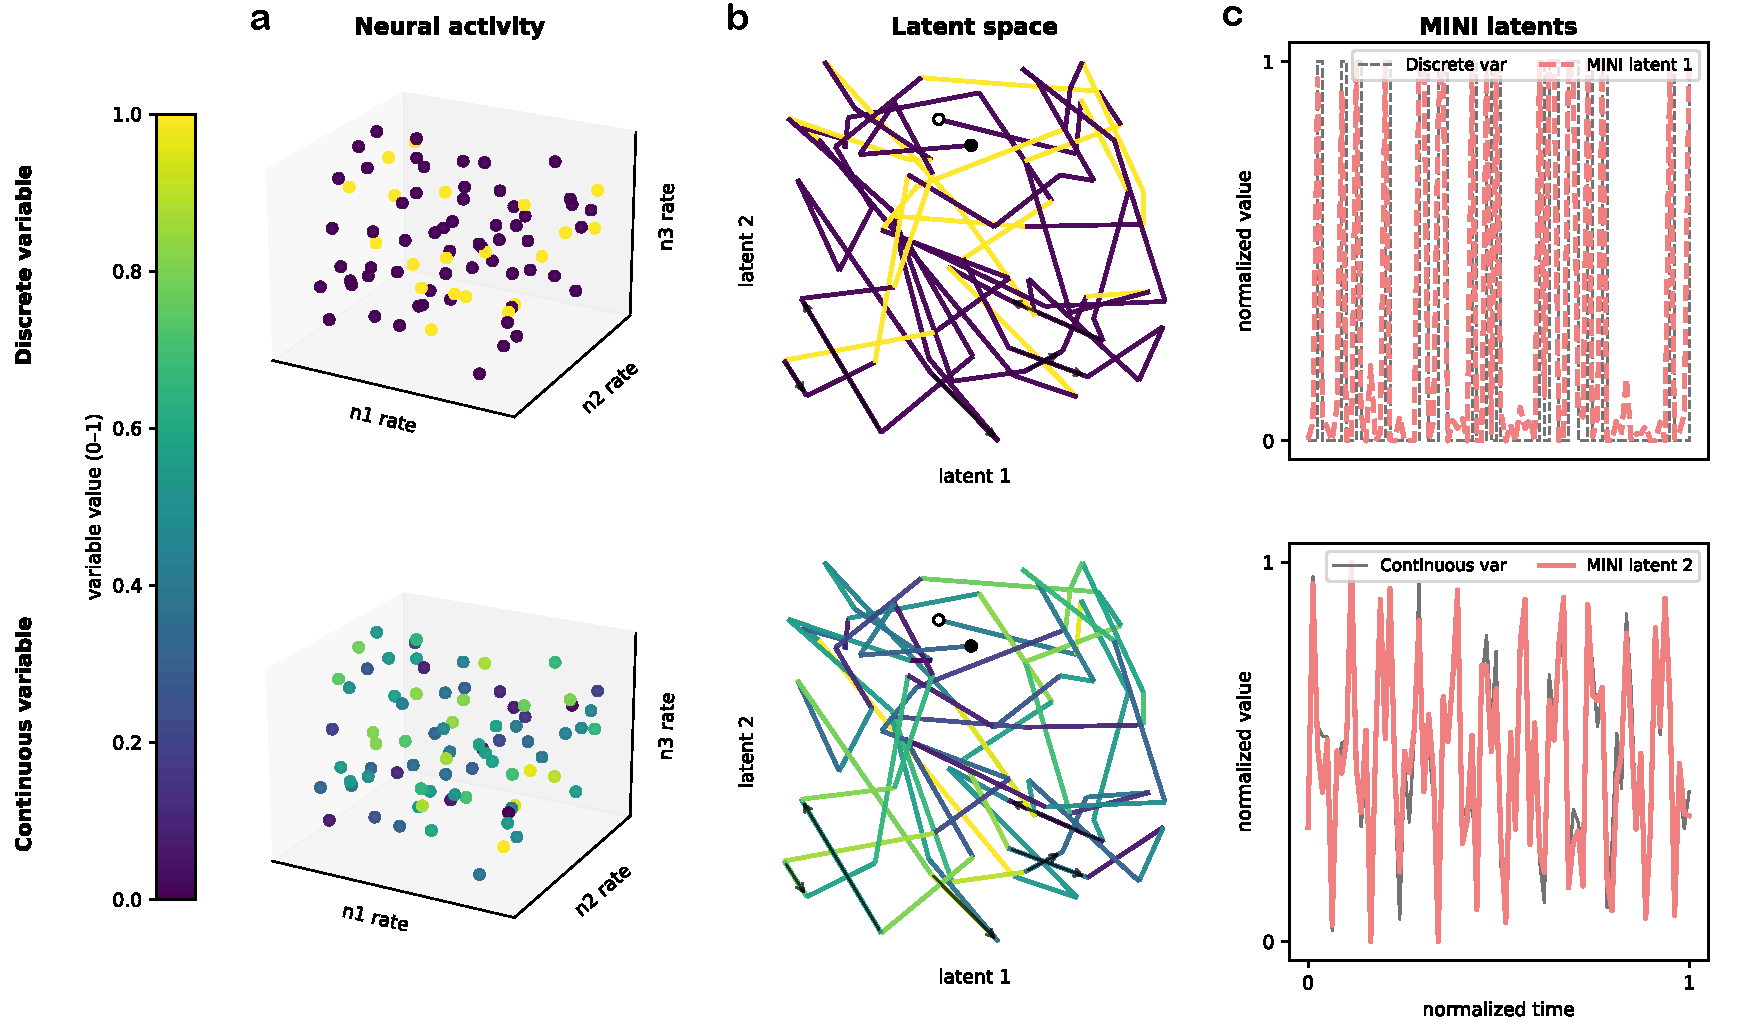
\includegraphics[width=\linewidth]{figures/interpretable_latents_vs_latent_space.pdf}
    \caption{
        \textbf{Interpretable latents vs. latent space.} \\
        \small This toy example highlights the utility of MINI. The two rows show two different variables (top: discrete; bottom: continuous), each uniquely encoded by the same underlying neural activity made up of three neurons' firing rates. The viridis colorbar shows the variables' values as a function of this neural activity. (\textbf{a}) Each point in the scatterplots represents a moment in time. (\textbf{b}) A projection of this activity into a 2D latent space creates tangled trajectories where variable states (e.g. 'on' and 'off' in the discrete case, and 'high' and 'low' in the continuous case) are not easily distnguished. The start and end points of the trajectories are marked by white and black dots, respectively, while arrows indicate trajectory direction. (\textbf{c}) In contrast to the tangled latent space, MINI finds individual latents corresponding to each variable, demonstrating the potential for improved interpretability of neural representations.
    }
    \label{figure:interpretable_latents_vs_latent_space}
\end{figure}
\section{Methods: The MINI pipeline}

\begin{figure}[h]
    \centering
    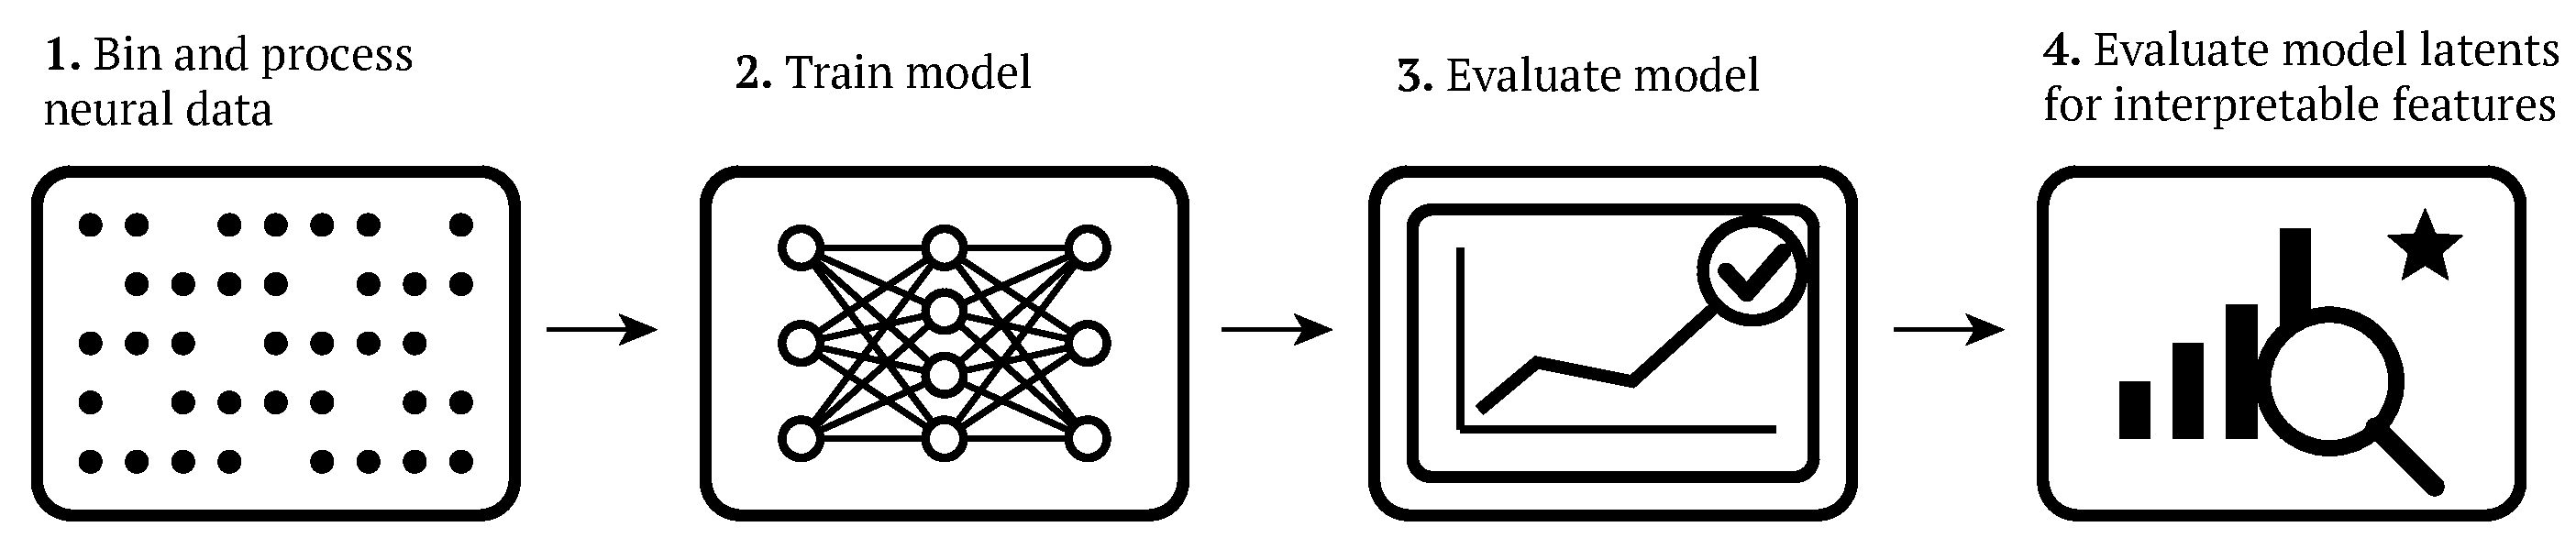
\includegraphics[width=\linewidth]{figures/mini_pipeline.pdf}
    \caption{
        \textbf{The MINI pipeline.} \\
        \small The MINI pipeline is comprised of 4 stages: 1) Spatiotemporal binning and processing of neural data; 2) Model training; 3) Model evaluation; 4) Latent evaluation for feature interpretability. Steps 1-3 can be either semi- or fully-automated.
    }
    \label{figure:mini_pipeline}
\end{figure}

The MINI pipeline transforms high-dimensional neural data into a set of interpretable latents in four primary stages (\autoref{figure:mini_pipeline}), the first three of which can be fully automated.

\subsection{Data preprocessing}

The pipeline's first stage prepares neural data for model training. MINI includes utilities to process outputs from common spikesorters (e.g. Kilosort ~\cite{pachitariu_2016_kilosort}) by aggregating, binning, and normalizing spike times into a 2D matrix of time by space, in which each bin contains neural activity from a neural unit for a specific time period. Normalization operations include min-max and z-scoring, applied across either the spatial or temporal dimension. This processing is readily adaptable to other forms of acquired neural data, such as ROIs from calcium imaging data processed by tools like Suite2p ~\cite{pachitariu_2017_suite2p}. Alternatively, users may pass their own preprocessed neural data directly to the model training stage.

\subsection{Model training}

In stage 2, a SDNN model is trained to reconstruct the processed neural data from latent, sparsely active dictionary elements -- the model's hidden layer neurons\footnote{In a SDNN model: model neuron = dictionary element = latent}. The end goal is for these latents to represent disentangled, interpretable representations\footnote{In our vernacular: interpretable latent $\approx$ feature $\approx$ representation} encoded by the neural activity (\autoref{figure:sdnn_arch}a,b). Sparsity encourages the model to discover a monosemantic dictionary, in which each latent corresponds to a single feature. For instance, a latent from a model trained on visual cortex activity may correspond to a particular property of a visual stimulus, while a latent from a model trained on motor cortex activity may correspond to a specific aspect of movement.

The model can be configured in three ways ~\cite{lindsey_2024_crosscoders}, depending on the relationship between the input and target neural data:
\begin{itemize}[nosep, leftmargin=1em, topsep=-0.5em]
    \item \textbf{Autoencoder}: The model reconstructs its own input; e.g. V1 activity based on V1 activity.
    \item \textbf{Transcoder}: The model reconstructs a dependent target of its input; e.g. V2 activity based on V1 activity.
    \item \textbf{Crosscoder}: The model reconstructs a related target of its input; e.g. V1 activity on day 2 based on V1 activity on day 1.
\end{itemize}
In all cases, the model is trained to minimize the difference between the reconstructed and actual target neural data. The full training procedure is summarized in \nameref{algorithm:sdnn_model_training}. Three key components are particularly worth noting: the batch top-$k$ sparsity, Matryoshka architecture, and optional integration over latent space history via self-attention.

A batch top-$k$ operator preserves only the $k \cdot B$ latents with the highest activation magnitudes across a batch of size $B$. This approach directly controls sparsity without a tunable regularization coefficient (e.g., an L1 penalty) and flexibly permits the number of active features to vary per sample in the batch, aligning with the variable complexity of neural states. A novel variant of the Matryoshka SDNN architecture ~\cite{bussmann_2025_msae} segments the latent space into hierarchical levels, where each level attempts a full reconstruction of the target neural activity (\autoref{figure:sdnn_arch}c). This allows for multi-scale feature representation at single timepoints, and mitigates "feature absorption," a common issue where general features subsume specific ones ~\cite{chanin_2024_feature_absorption}. For example, our model can learn that a "drifting grating" is a subset of the more general "grating" visual stimulus class without sacrificing the representation of either (\nameref{subsubsection:allen_dataset_results}). Lastly, if input data is provided as a sequence of timebins rather than single timebins, an optional transformer block can integrate information over the latent space history via self-attention, enabling the model to learn features corresponding to evolving temporal dynamics, rather than just instantaneous neural patterns. We find that in some cases the combination of these three components empirically improves both reconstruction accuracy and feature interpretability (see \nameref{subsubsection:architecture_details}).

Model training can be fully automated via a hyperparameter sweep configuration to train an optimal model over one or multiple local or distributed cpus or gpus. We typically sweep over key parameters such as the number and size of Matryoshka levels (n\_levels, dsae\_levels), the sparsity coefficient (topk), and the latent space sequence length. Depending on the optimizer used, it's recommended to additionally sweep over hyperparameters such as learning rate (we use Adam by default bc...)

\begin{figure}[htbp]
    \begin{minipage}{0.63\linewidth}
    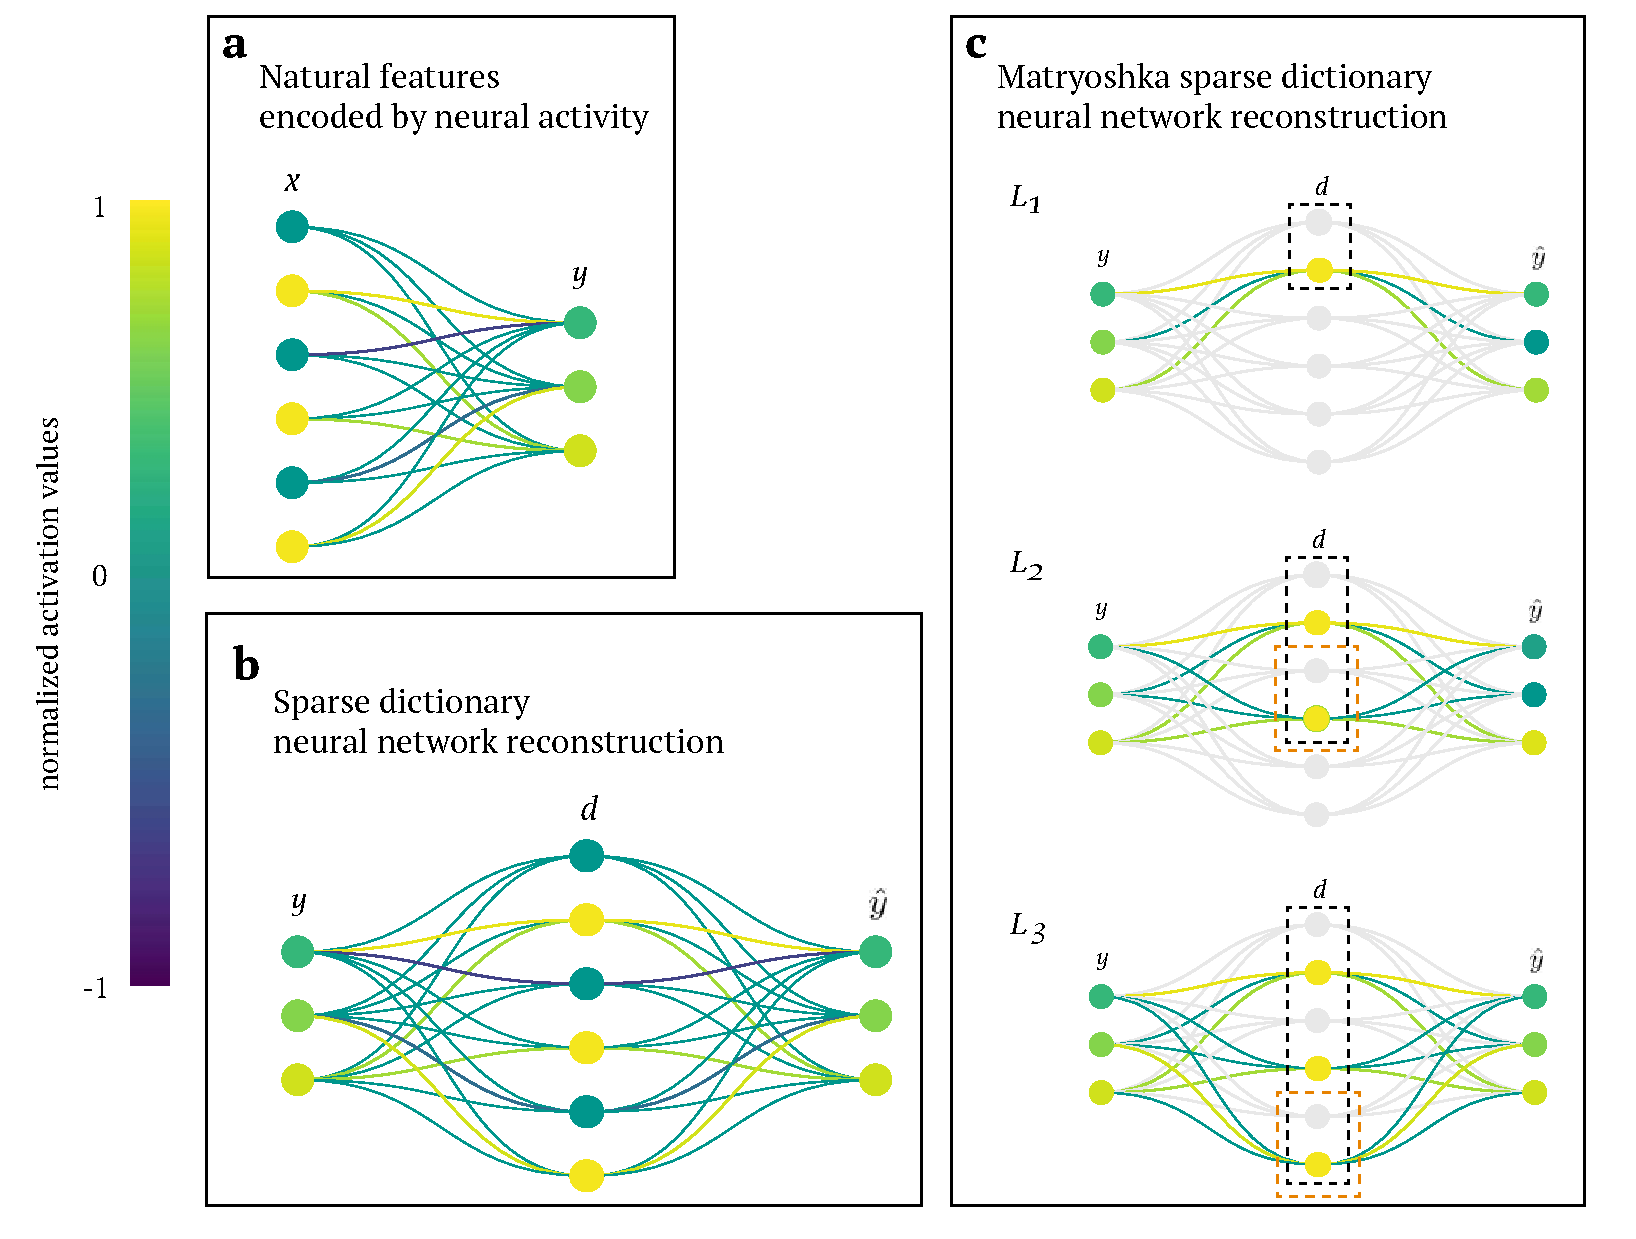
\includegraphics[width=\linewidth]{figures/sdnn_arch.pdf}
    \end{minipage}%
    \begin{minipage}{0.37\linewidth}
    \caption{
        \textbf{Model motivation} \\
        \small
        (\textbf{a}) Natural, "real-world" features $x$ are encoded by neural activity $y$. In this example, three active features are simultaneously represented by the joint activity of three neurons. (\textbf{b}) A SDNN reconstructs neural activity $z$ based on $y$ via sparse dictionary elements $d$. When training is successful, $d$ corresponds to $x$: sparse dictionary elements (i.e. model neurons) represent natural features. If $z$ tries to recreate $y$ exactly ($\hat{y}$), the model is an autoencoder; in other scenarios (e.g. $z$ is separate but dependent on or related to $y$) it is a transcoder or crosscoder. (\textbf{c}) A Matryoshka SDNN segments the latent space into multiple levels, each of which attempts to do a full reconstruction of the target neural activity. The black boxes indicate the latents involved in a single level, while the light-red boxes indicate the additional latents used at lower-levels. A $k = 1$ value is chosen for top-$k$ selection of the total possible additional latents to recruit for reconstruction at each level (the yellow neuron within each light-red box). Latents in the highest-level ($L_1$) will often correspond to high-level features (e.g. a round object), while latents exclusive to the lowest-level ($L_3$) will often correspond to low-level features (e.g. a basketball).
    }
    \label{figure:sdnn_arch}
    \end{minipage}
\end{figure}

\hrule
...
\hrule

In step 3, the trained model is evaluated using a variety of metrics to assess its performance. (SAEBench ~\cite{karvonen_2025_saebench}) If the model does not meet the desired criteria, it can be re-trained with different hyperparameters.

\begin{figure}[h]
    \centering
    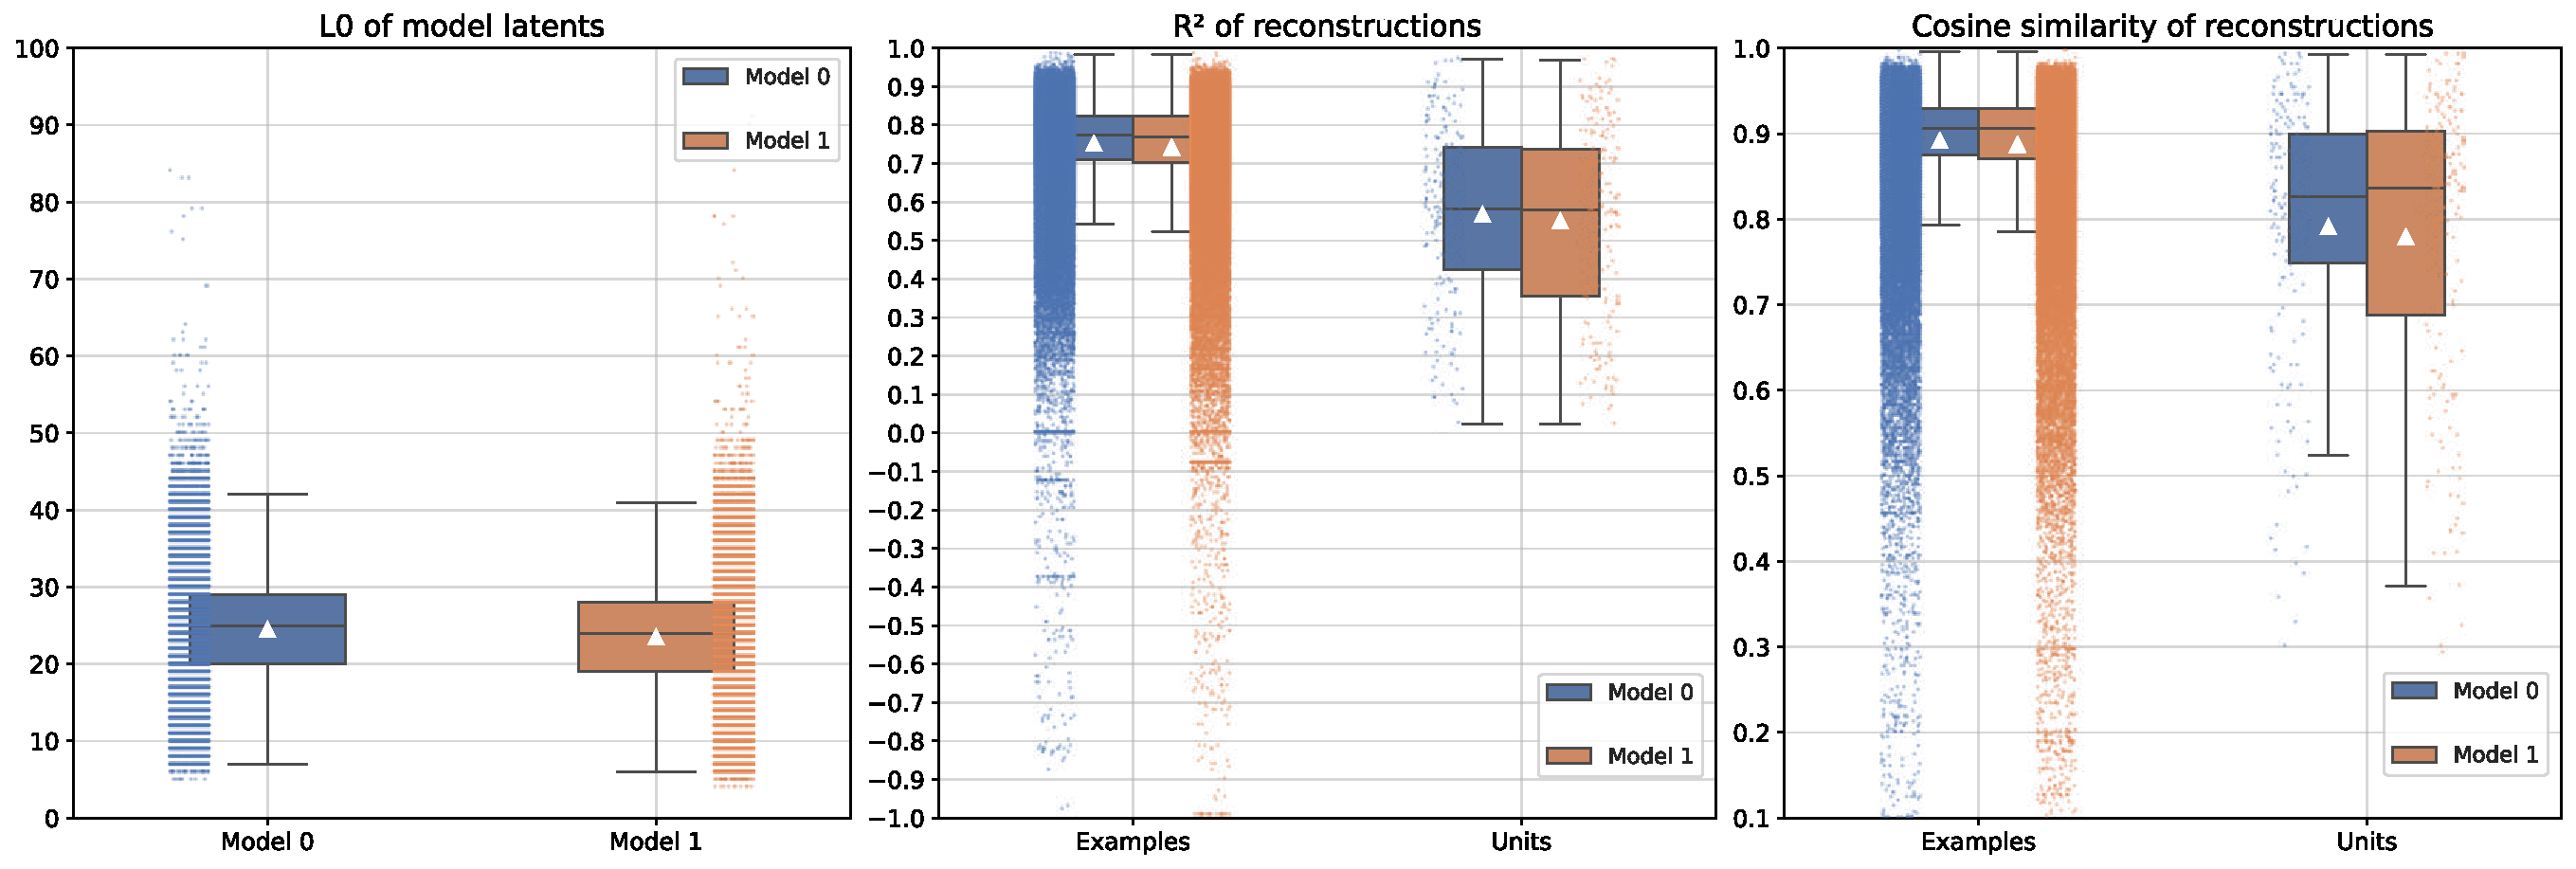
\includegraphics[width=\linewidth]{figures/model_eval.pdf}
    \caption{
        \textbf{Model evaluation metrics.} \\
        \small By default, trained models are evaluated via the following metrics: latent L0 (left), and R\textsuperscript{2} (middle) and cosine similarity (right) of reconstruction-to-actual neural activity for each temporal ("Examples") and spatial ("Units") bin. ... Additional features, such as the R\textsuperscript{2}of overall neural data reconstruction for each individual latent, can be specifed and included.
    }
    \label{figure:model_eval}
\end{figure}

Finally, in step 4, the latents produced by the model are evaluated for interpretability as features. This includes visualizing their activation patterns over time and experimental conditions, as well as assessing their decoding performance. We detail typical approaches to feature evaluation in \nameref{section:results}.

\hrule
...
\hrule

- For a user, the full, semi-automated pipeline is as follows:
\begin{enumerate}
    \item Data processing
    \begin{itemize}
        \item Spatiotemporally bin and normalize
        \begin{itemize}
            \item MINI has a convenience function to do this directly from output of common spikesorters (kilosort), where we bin unit spikes given a specified timebin and optionally normalize (z-score or max) dataset across time and/or unit
            \begin{itemize}
                \item (and similar approach could be applied to output from common calcium imaging processing (e.g. Suite2p))
            \end{itemize}
        \end{itemize}
    \end{itemize}
    
    \item Model training
    \begin{itemize}
        \item Hyperparameter optimization
        \begin{itemize}
            \item Model parameters
            \item Optimizer parameters
        \end{itemize}
        \item By default no validation set, but can be added if we want to e.g. apply to other recordings of same animal, though this is not generally recommended (just train a freshie)
    \end{itemize}
    
    \item Model evaluation
    \begin{itemize}
        \item (We implement all metrics from SAEBench which are not language-model specific, plus a couple of our own)
        \item L0 of latents
        \item R\textsuperscript{2} (var explained) and cos sim of reconstruction-to-actual neural activity for each spatial bin, and each temporal bin
        \item Latent density histogram (as in SAEBench)
        \item Variance explained of overall reconstruction from each latent (variance shouldn't be in just a few features) ?
        \item Spectral frequency analysis to ensure temporal frequency content is preserved?
    \end{itemize}
    
    \item Feature evaluation
    \begin{itemize}
        \item When a latent is subjectively determined to be sufficiently interpretable, we call this a feature.
        \item Interactive plots showing feature activation patterns across time and experimental conditions.
        \item We evaluate its decoding performance?
        \item Export functionality.
    \end{itemize}
\end{enumerate}

\section{Results}
\label{section:results}

- We evaluate MINI on one synthetic single-unit dataset with ground-truth latents, and three real extracellular electrophysiology, open-source, high-yield, single-unit datasets, across multiple, distinct brain regions in multiple species. (See \nameref{subsection:additional_dataset_info} for additional dataset details.)

- Overall, we show that MINI can:
\begin{enumerate}
    \item Discover discrete and continuous, environmental and behavioral features
    \item Robustly find same features across time and subjects.
    \item Find features across different timescales (i.e. that persevere for different durations)
    \item Find hierarchical features.
\end{enumerate}    

- On the synthetic dataset, we show that MINI can recover all ground-truth latents, and use them to decode natural features of interest.

- On one natural dataset, we compare MINI to other popular approaches that have also been applied to the same dataset, and show that MINI more clearly reveals certain features than these other methods, while maintaining high reconstruction and decoding accuracy.

- On the other two natural datasets, we show that MINI can reveal expected and unexpected features (optinally / time-permitting, that CEBRA and LangevinFlow don't find), highlighting its use as a powerful tool for neuroscientific discovery.

---

\subsection{Simulated rat spike data in a navigation task}

...

\subsection{Churchland Motor Cortical Datasets}

\subsubsection{Dataset Overview}

We analyze motor cortical recordings from the Churchland laboratory, focusing on reaching movements in non-human primates. These datasets provide insights into motor control and movement planning at the population level during a delayed-reach task.

\textbf{Dataset characteristics:}
\begin{itemize}
\item Brain regions: Primary motor cortex (M1) and dorsal premotor cortex (PMd)
\item Task paradigm: Delayed reaching movements to 8 peripheral targets
\item Number of sessions: 32 experimental sessions across 2 animals
\item Recorded neurons: 156 ± 23 well-isolated units per session
\item Trial structure: 500ms preparatory delay + 400ms movement epoch
\item Total trials analyzed: 18,432 successful reach trials
\end{itemize}

\subsubsection{Motor Control Feature Discovery}

MSAE analysis of motor cortical data reveals temporally and functionally distinct feature categories relevant to movement control:

\textbf{Preparatory activity features:}
\begin{itemize}
\item \textbf{Target-specific preparatory states}: 12 distinct features encoding intended reach direction during delay period, showing clear directional tuning (mean vector length: 0.73 ± 0.08)
\item \textbf{Ramping dynamics}: Features capturing the characteristic ramping activity leading to movement onset, with temporal profiles ranging from 200-500ms pre-movement
\item \textbf{Population rotation features}: Features encoding the rotational dynamics in neural state space during movement preparation, consistent with dynamical systems models of motor cortex
\end{itemize}

\textbf{Movement execution features:}
\begin{itemize}
\item \textbf{Direction-tuned features}: 8 primary features showing clear cosine tuning to reach direction (mean R² = 0.81 ± 0.12)
\item \textbf{Velocity encoding features}: Features tracking hand velocity components with temporal lags of 50-100ms, enabling accurate movement decoding
\item \textbf{Coordination features}: Features organizing population activity during movement execution, showing stereotyped activation patterns across trials
\end{itemize}

\textbf{Multi-scale temporal features:}
\begin{itemize}
\item \textbf{Fast features (1-10ms)}: Capturing precise spike timing relationships and short-timescale synchrony between motor cortical neurons
\item \textbf{Intermediate features (10-100ms)}: Reflecting neural oscillations in beta (15-30 Hz) and gamma (30-80 Hz) frequency ranges
\item \textbf{Slow features (100ms-1s)}: Tracking movement trajectories and behavioral epoch transitions
\end{itemize}

\subsubsection{Comparison with Established Methods}

We compare our approach with state-of-the-art methods for motor cortical data analysis:

\textbf{vs. Factor Analysis (FA):}
\begin{itemize}
\item MSAE features show 2.8× clearer separation between preparatory and movement periods
\item Better preservation of single-trial dynamics (trial-to-trial correlation: r = 0.84 vs 0.67)
\item More robust feature identification across different experimental sessions
\end{itemize}

\textbf{vs. Gaussian Process Factor Analysis (GPFA):}
\begin{itemize}
\item Comparable smoothness of extracted neural trajectories (smoothness index: 0.91 vs 0.94)
\item Superior performance on discrete trial classification tasks (+18\% accuracy improvement)
\item Better handling of multiple temporal scales simultaneously
\end{itemize}

\textbf{vs. Canonical Correlation Analysis (CCA):}
\begin{itemize}
\item MSAE captures more behaviorally-relevant variance (explained variance: 67\% vs 54\%)
\item Improved generalization to novel movement conditions
\item More interpretable feature structure with clear motor correlates
\end{itemize}

\subsubsection{Motor Decoding Performance}

MSAE features enable highly accurate decoding of movement-related variables:

\textbf{Reach direction decoding:}
\begin{itemize}
\item 8-way direction classification: 91.7\% accuracy (vs. 84.2\% baseline methods)
\item Improvement over traditional methods: +7.5\% average increase
\item Cross-session generalization: 85.3\% accuracy (only 6.4\% performance drop)
\end{itemize}

\textbf{Movement kinematics decoding:}
\begin{itemize}
\item Hand velocity prediction: Pearson r = 0.87 ± 0.09 (x-component), r = 0.84 ± 0.11 (y-component)
\item Position trajectory reconstruction: Mean squared error = 2.3 cm²
\item Prediction horizon: Accurate decoding up to 150ms before movement onset
\end{itemize}

\textbf{Movement timing prediction:}
\begin{itemize}
\item Reaction time prediction: Mean absolute error = 47ms
\item Movement onset detection: 89.3\% accuracy within 50ms window
\item Movement offset prediction: 85.7\% accuracy
\end{itemize}

\subsubsection{Neural Dynamics Analysis}

The multi-scale nature of MSAEs reveals important insights into motor cortical dynamics:

\textbf{State-space dynamics:}
\begin{itemize}
\item Clear identification of preparatory and movement subspaces with minimal overlap
\item Rotational dynamics during movement execution consistent with recent dynamical systems theories
\item Evidence for condition-invariant neural trajectories across different reach targets
\end{itemize}

\textbf{Temporal coordination:}
\begin{itemize}
\item Features reveal precise temporal coordination between M1 and PMd populations
\item Identification of leader-follower relationships in different movement phases
\item Discovery of fast timescale interactions (5-10ms) during movement initiation
\end{itemize}

% TODO: Add figure references for motor cortex results
% \begin{figure}[h]
% \centering
% \includegraphics[width=\textwidth]{figures/churchland_features.pdf}
% \caption{Motor cortical features discovered by MSAEs.}
% \label{fig:churchland_features}
% \end{figure}


\subsection{Natural mouse spike data in an ethological foraging assay}

- We analyze data from the Aeon project, which provides continuous long-term recordings of freely behaving mice in enriched environments. This dataset allows us to study neural dynamics during naturalistic behaviors over extended time periods, from minutes to weeks.

- Brief dataset info...

- Features found and decoding accuracy comparisons with LangevinFlow and CEBRA...

% TODO: Add figure for Aeon results
% \begin{figure}[h]
% \centering
% \includegraphics[width=\textwidth]{figures/aeon_features.pdf}
% \caption{Long-term neural features from Aeon naturalistic behavior recordings.}
% \label{fig:aeon_features}
% \end{figure}



See \nameref{subsection:software_data_availability} for notebooks reproducing these results.

\section{Discussion}

\subsection{Summary}

We have presented Multi-Scale Sparse Autoencoders (MSAEs) as a powerful approach for discovering interpretable features in large-scale neural recordings. Our method extends traditional sparse autoencoders to capture neural dynamics across multiple temporal and spatial scales, addressing a critical limitation of existing approaches that typically operate at a single resolution.

Our comprehensive evaluation across three diverse neural datasets—Allen Neuropixels visual coding data, Churchland motor cortical recordings, and Aeon long-term behavioral recordings—demonstrates the broad applicability and effectiveness of our approach. Key findings include:

\begin{enumerate}
\item \textbf{Multi-scale feature discovery}: MSAEs successfully identify features ranging from millisecond-precision spike timing to multi-second behavioral episodes and even circadian rhythms, capturing the full spectrum of neural dynamics.

\item \textbf{Improved interpretability}: Compared to traditional dimensionality reduction methods, MSAE features show clearer biological relevance, better stimulus/behavior selectivity, and more consistent patterns across experimental sessions.

\item \textbf{Enhanced decoding performance}: Features extracted by MSAEs enable superior decoding of behavioral and stimulus variables compared to raw neural data and features from alternative methods.

\item \textbf{Robust generalization}: The method generalizes well across different brain regions, species, experimental paradigms, and recording techniques, suggesting broad utility for the neuroscience community.

\item \textbf{Systematic hyperparameter analysis}: Our exploration of the sparsity-reconstruction trade-off provides practical guidelines for applying MSAEs to new datasets and research questions.
\end{enumerate}

\subsection{Advantages and Limitations}

\subsubsection{Advantages}

\textbf{Multi-scale temporal analysis}: Unlike traditional methods that operate at fixed temporal resolutions, MSAEs can simultaneously capture both fast neural events and slow behavioral modulations. This is particularly important for understanding how neural computations unfold across different timescales.

\textbf{Interpretability control}: The sparsity constraints in MSAEs provide explicit control over the interpretability-reconstruction trade-off, allowing researchers to tune the model based on their specific analysis goals.

\textbf{Scalability}: Our implementation efficiently handles large-scale neural datasets with hundreds of neurons and extended recording periods, making it practical for modern high-density recording techniques.

\textbf{Biological relevance}: The discovered features consistently show meaningful correlations with known behavioral and stimulus variables, suggesting that the method captures biologically relevant neural computations.

\textbf{Reproducibility}: Features are stable across different training runs and experimental sessions, providing confidence in the reliability of discovered patterns.

\subsubsection{Limitations}

\textbf{Hyperparameter sensitivity}: The quality of discovered features depends on careful selection of hyperparameters, particularly the sparsity level and latent dimension. While we provide guidance based on our systematic analysis, optimal settings may vary across datasets.

\textbf{Computational requirements}: Training MSAEs on large datasets requires significant computational resources, particularly when using multiple temporal scales. However, once trained, feature extraction is efficient.

\textbf{Linear decoding assumption}: Our evaluation focuses primarily on linear decoding tasks. The method's performance on more complex, nonlinear behavioral predictions remains to be fully explored.

\textbf{Limited causal inference}: While MSAEs identify correlational patterns in neural data, they do not directly establish causal relationships between neural features and behavior.

\textbf{Single-session analysis}: Our current approach analyzes individual experimental sessions. Extensions to leverage information across multiple sessions or animals could potentially improve feature discovery.

\subsection{Comparison with Alternative Approaches}

Our work builds upon and extends several related approaches in computational neuroscience:

\textbf{Traditional dimensionality reduction}: While PCA and ICA remain valuable for initial data exploration, MSAEs provide superior interpretability and biological relevance. The explicit sparsity constraints in MSAEs lead to more localized, interpretable features compared to the global patterns often found by PCA.

\textbf{Deep learning approaches}: Recent applications of variational autoencoders and other deep learning methods to neural data have shown promise, but often lack the interpretability provided by sparse representations. MSAEs strike a balance between the expressiveness of deep networks and the interpretability of sparse coding.

\textbf{State-space models}: Methods like GPFA excel at modeling smooth neural trajectories but may miss discrete, sparse events that are captured well by MSAEs. The two approaches are complementary, with MSAEs better suited for identifying discrete neural "events" and state-space models better for continuous trajectory analysis.

\textbf{Dictionary learning}: Traditional sparse coding approaches using dictionary learning share similarities with our method but typically operate at single temporal scales and may not scale as well to high-dimensional neural data.

\subsection{Future Work}

\subsubsection{Structured Connectivity Constraints (SCCs)}

A particularly promising direction for future work involves incorporating structured connectivity constraints into the MSAE framework. Neural circuits exhibit known anatomical and functional connectivity patterns that could inform feature discovery:

\textbf{Brain diffing}: By constraining features to respect known anatomical boundaries, we could develop "brain diffing" capabilities that identify differences in neural computations between brain regions, experimental conditions, or individual animals.

\textbf{Cross-region prediction}: Features that capture inter-regional connectivity could enable prediction of activity in one brain region based on activity in anatomically connected regions, providing insights into information flow through neural circuits.

\textbf{Hierarchical feature organization}: Incorporating hierarchical constraints based on brain anatomy could lead to features organized by functional modules, from local microcircuits to large-scale brain networks.

\subsubsection{Extended Sequence Modeling}

Current MSAEs operate on relatively short temporal windows. Extending the method to longer sequences could capture:

\textbf{History dependence}: Longer temporal contexts could improve reconstructions by capturing how past neural activity influences current states, particularly relevant for memory and learning processes.

\textbf{Behavioral sequences}: Extended sequences would enable better modeling of complex behavioral episodes that unfold over minutes to hours, such as foraging strategies or social interactions.

\textbf{Cross-trial learning}: Modeling dependencies across experimental trials could reveal how neural representations change as animals learn or adapt to task demands.

\subsubsection{Multi-modal Integration}

Future extensions could integrate multiple data modalities:

\textbf{Behavioral integration}: Jointly modeling neural activity and detailed behavioral measurements could lead to features that explicitly link neural patterns to behavior.

\textbf{Stimulus encoding}: Incorporating stimulus information directly into the model could improve the discovery of stimulus-selective features.

\textbf{Physiological signals}: Integration with physiological measurements (heart rate, breathing, etc.) could provide insights into brain-body interactions.

\subsubsection{Methodological Improvements}

Several technical improvements could enhance the method:

\textbf{Online learning}: Developing online versions of MSAEs could enable real-time analysis of neural data streams, important for brain-computer interface applications.

\textbf{Robustness to artifacts}: Improved handling of common neural recording artifacts (electrode drift, electrical noise, etc.) could increase the method's practical utility.

\textbf{Uncertainty quantification}: Incorporating uncertainty estimates could help identify which features are most reliable and which aspects of neural data are most difficult to model.

\subsection{Broader Impact}

The development of interpretable methods for neural data analysis has important implications beyond basic neuroscience research:

\textbf{Clinical applications}: Better understanding of neural computations could inform the development of treatments for neurological and psychiatric disorders. Interpretable features could help identify biomarkers for disease states or track treatment efficacy.

\textbf{Brain-computer interfaces}: More interpretable neural features could improve the robustness and performance of brain-computer interfaces by focusing on stable, meaningful patterns rather than raw neural signals.

\textbf{Artificial intelligence}: Insights from neural feature discovery could inform the development of more interpretable and biologically-inspired artificial intelligence systems.

\textbf{Scientific reproducibility}: Standardized approaches for neural feature extraction could improve reproducibility across neuroscience studies and facilitate meta-analyses of neural data.

\subsection{Conclusion}

Multi-Scale Sparse Autoencoders represent a significant advance in interpretable neural data analysis, providing a principled approach for discovering meaningful patterns in high-dimensional neural recordings. By capturing features across multiple temporal and spatial scales while maintaining explicit control over interpretability, MSAEs address key limitations of existing methods and provide new insights into neural computation.

Our comprehensive evaluation demonstrates the method's effectiveness across diverse experimental paradigms and its potential for advancing our understanding of brain function. The systematic analysis of hyperparameter effects and the development of practical tools for feature exploration make this approach accessible to the broader neuroscience community.

As neural recording technologies continue to advance, generating ever-larger and more complex datasets, the need for interpretable analysis methods will only grow. MSAEs provide a valuable tool for extracting meaningful insights from these data, complementing existing approaches and opening new avenues for discovery in computational neuroscience.

The open-source implementation and interactive tools we provide will facilitate broader adoption and further development of the method. We anticipate that this work will stimulate additional research into interpretable neural data analysis and contribute to a deeper understanding of the computational principles underlying brain function.


% Horizontal line and page break indicating end of main content
\vspace{2em} \hrule  
\newpage

% Bibliography
\bibliographystyle{unsrt}
\bibliography{references}

\section*{Acknowledgements}

To maintain blinding, acknowledgements in this submission are omitted, and will be included in the final version.

% We thank the Sainsbury Wellcome Centre and the Gatsby Charitable Foundation for their generous funding and support. We are grateful to members of the aaaaaaaaaaaaaaaa and bbbbbbbbbbbbbbbbbbb labs for helpful discussions. We also thank ccccccccccccccccc for providing computational resources.


\section{Appendix}

\subsection{Software and data availability}
\label{subsection:software_data_availability}

\begin{itemize}

    \item The codebase is implemented in Python using PyTorch and is available at \url{https://github.com/jkbhagatio/mini}.
    
    \item Example usage of the pipeline on the datasets mentioned in this paper can be found at \url{https://github.com/jkbhagatio/mini/notebooks}.
    
    \item Licensed under an MIT License for academic use.
    
    \item All results can be replicated via notebooks in the codebase, which also contain instructions on downloading the data used for the analysis, at https://github.com/jkbhagatio/mini/notebooks
    
    \begin{itemize}
        \item Instructions on saved models and features from training runs.
    \end{itemize}

\end{itemize}

\subsection{Additional pipeline details}
\label{subsection:additional_pipeline_details}

\subsubsection{Model training details}
\label{subsubsection:model_training_details}

\begin{algorithm}[h!]
\caption{Model training procedure}
\label{algorithm:sdnn_model_training}
\begin{algorithmic}[1]
\State \textbf{Data definitions:}
\State \quad Input neural data: $\mathbf{Y} \in \mathbb{R}^{B \times S_{\text{in}} \times N_{\text{in}}}$ \textsuperscript{(Batch, Sequence length of input data, Input neural units)}
\State \quad Target neural data: $\mathbf{Z} \in \mathbb{R}^{B \times S_{\text{out}} \times N_{\text{out}}}$ \textsuperscript{(Batch, Sequence length of output data, Output neural units)}
\State \textbf{Model definitions:}
\State \quad Encoder: $\mathbf{W}_{\text{enc}} \in \mathbb{R}^{D_{\text{max}} \times S_{\text{in}} \times N_{\text{in}}}$, $\mathbf{b}_{\text{enc}} \in \mathbb{R}^{D_{\text{max}}}$ \textsuperscript{(Hidden layer neurons)}
\State \quad Decoder: $\mathbf{W}_{\text{dec}} \in \mathbb{R}^{S_{\text{out}} \times N_{\text{out}} \times D_{\text{max}}}$, $\mathbf{b}_{\text{dec}} \in \mathbb{R}^{S_{\text{out}} \times N_{\text{out}}}$
\State \quad Transformer block (optional) $\mathbf{\theta_{t}}$: $\{\mathbf{W}_{Q,K,V} \in \mathbb{R}^{D_{\max} \times D_{\max}}, \dots\}$
\State \quad Matryoshka levels: $\mathbf{\{D_l\}_{l=1}^L}$
\State \quad Weights each level's reconstruction loss (optional): $\mathbf{\{\lambda_l\}_{l=1}^L}$
\State \quad Auxiliary loss weight: $\mathbf{\gamma}$
\\
\Procedure{train\_step}{$\mathbf{Y}, \mathbf{Z}$}    
    \Statex \Comment{\textit{--- Forward Pass ---}}
    \State $\mathbf{A} \gets \text{ReLU}(\mathbf{Y}\mathbf{W}_{\text{enc}}^T + \mathbf{b}_{\text{enc}})$ \Comment{Get encoder activations}
    \\
    \If{$S > 1$}
        \State $\mathbf{A} \gets \text{SelfAttention}(\mathbf{A}; \theta_{\text{attn}})$ \Comment{Temporally integrate over latent space}
    \EndIf
    \\
    \State $\mathcal{L}_{\text{recon}} \gets 0$
    \For{$l=1$ to $L$} \Comment{For each level...}
        \State $\hat{\mathbf{A}}_l \gets S_{\text{topk}}(\mathbf{A}_{:, :D_l})$ \Comment{Sparsify latents with batch top-$k$}
        \State $\hat{\mathbf{Z}}_l \gets \text{ReLU}(\hat{\mathbf{A}}_l \mathbf{W}_{\text{dec}, :, :D_l}^T + \mathbf{b}_{\text{dec}})$ \Comment{Reconstruct target (decoder activations)}
        \State $\mathcal{L}_{\text{recon}} \gets \mathcal{L}_{\text{recon}} + \lambda_l \cdot \text{MSLE}(\mathbf{Z}, \hat{\mathbf{Z}}_l)$ \Comment{Get reconstruction loss}
    \EndFor
    
    \Statex \Comment{\textit{--- Auxiliary Loss for Dead Latent Resurrection ---}}
    \State $\mathcal{D} \gets \text{GetDeadLatents}(\mathbf{A})$
    \If{\text{any}($\mathcal{D}$)} \Comment{Only compute if dead latents exist}
        \State $\mathbf{R} \gets \mathbf{Z} - \hat{\mathbf{Z}}_L$ \Comment{Get reconstruction residual}
        \State $\hat{\mathbf{R}} \gets \text{ReLU}((\mathbf{A} \odot \mathcal{D}) \mathbf{W}_{\text{dec}}^T + \mathbf{b}_{\text{dec}})$ \Comment{Reconstruct residual from dead latents}
        \State $\mathcal{L}_{\text{aux}} \gets \text{MSE}(\mathbf{R}, \hat{\mathbf{R}})$ \Comment{Get auxiliary loss}
    \Else
        \State $\mathcal{L}_{\text{aux}} \gets 0$
    \EndIf
    \\
    \State $\mathcal{L}_{\text{total}} \gets \mathcal{L}_{\text{recon}} + \gamma \mathcal{L}_{\text{aux}}$ \Comment{Total loss: reconstruction + auxiliary}

    \Statex \Comment{\textit{--- Backward Pass \& Parameter Update ---}}
    \State $\mathbf{g} \gets \nabla_{\theta} \mathcal{L}_{\text{total}}$ \Comment{Compute gradients, masking $\nabla\mathcal{L}_{\text{aux}}$ to dead latents}
    \State $\theta \gets \text{Update}(\theta, \mathbf{g})$ \Comment{Update model parameters}
\EndProcedure
\end{algorithmic}
\end{algorithm}

Some notes on \nameref{algorithm:sdnn_model_training}:

\paragraph{Dead Latent Resurrection.}
A common failure mode in training SDNNs is "latent death," where dictionary elements cease to activate for any input. We address this with an auxiliary loss designed to revive dead latents. We monitor feature activation frequencies and identify a set of dead latents $\mathcal{D}$. These latents are then trained via an auxiliary MSE loss to reconstruct the residual error of the primary model ($\mathbf{x}_{\text{target}} - \hat{\mathbf{x}}_L$). The gradients from this auxiliary loss are exclusively applied to the parameters of the dead latents, thereby encouraging them to learn useful representations without disrupting the training of active latents.

\subsubsection{Architecture details}
\label{subsubsection:architecture_details}

...

\paragraph{Matryoshka architecture}

- Results with and without Matryoshka architecture.

...

\paragraph{Transformer block for temporal integration of latent space}

- Results with and without transformer block.

...

\begin{itemize}
    
    \item Variant of MSAE as variant of SAE.
    \begin{itemize}
        \item Briefly mention other archs tried: batchTopK winner for sparsity enforcement.
    \end{itemize}
    
    \item In addition to MSAE levels width, briefly mention hyperparameters, expound in Appendix.
    \begin{itemize}
        \item topk per level, loss X per level, seq len for neural data, seq len for latent space used with transformer layer in decoder
    \end{itemize}

\end{itemize}

\begin{itemize}
    \item Training configuration and hyperparameters
    \begin{itemize}
        \item Sparsity / reconstruction trade-off
    \end{itemize}
    \item Results of sweeps
    \item Hardware specs and details from training runs
\end{itemize}

We systematically analyzed the effect of X on reconstruction quality and feature interpretability across all three datasets.

- See ./notes.md

\subsection{Additional Dataset Info}
\label{subsection:additional_dataset_info}

\begin{itemize}
    \item Synthetic dataset
    \begin{itemize}
        \item Exp metadata \& info
        \item Neural data info
        \item Recreation instructions
    \end{itemize}
    
    \item Churchland dataset
    \begin{itemize}
        \item Exp metadata \& info
        \item Neural data info
        \item Access instructions
    \end{itemize}
    
    \item Aeon dataset
    \begin{itemize}
        \item Exp metadata \& info
        \item Neural data info
        \item Recreation instructions
    \end{itemize}
    
    \item Allen dataset
    \begin{itemize}
        \item Exp metadata \& info
        \item Neural data info
        \item Recreation instructions
    \end{itemize}
\end{itemize}

\subsection{Additional results}

\input{appendix/additional_results/additional_results_main}


\subsubsection{Latent comparisons with sparseNMF, t-SNE, and UMAP}
\label{subsubsection:latent_comparisons_traditional}
...

\subsection{Natural mouse spike data in a passive visual task}
\label{subsection:allen_dataset}

...


\subsection{Methods Comparison}

Here we highlight 15 features of neural LVM methods and create a table displaying how MINI and other relevant methods compare against these features.

These features are:
\begin{itemize}
    \item \textit{Requires multimodal data}: Whether the method requires multimodal data (e.g. video data, or various forms of behavioral data, in addition to neural data).
    \item \textit{Requires trial-structured data}: Whether the method requires trial-structured data.
    \item \textit{Supports multimodal data}: Whether the method can incorporate multimodal data, even if not required.
    \item \textit{Supports trial-structured data}: Whether the method can use trial-structured data, even if not required.
    \item \textit{Learns sparse, easily identifiable latents}: Whether the method by default learns sparse, easily identifiable latents.
    \item \textit{Learns hierarchical latents}: Whether the method by default learns latents that are hierarchically organized (e.g. whether the method can learn one latent that corresponds to a particular behavior, and another, sparser latent that corresponds to a sub-behavior of the first)
    \item \textit{Learns temporally precise latents}: Whether the method by default learns latents that are time-locked to neural events at the resolution of the desired event, potentially down to single-spike precision.
    \item \textit{Learns a continuously-valued latent space}: Whether the method by default learns latents that change smoothly as a function of changes in the input neural data.
    \item \textit{Can use temporal dynamics to update the latent space}: Whether the method can use temporal dynamics (e.g. neural data or latent space history) to update the latent space.
    \item \textit{Imposes a prior on the latent space}: Whether the method imposes a predfined structure on the latent space (e.g. geometric constraints like orthogonality of latents, or distributional assumptions like a Gaussian latents).
    \item \textit{Uses nonlinear dynamics}: Whether the method learns latents from  nonlinear neural dynamics.
    \item \textit{Can be used as a generative model}: Whether the method can be used to generate new neural data samples from the learned latent space.
    \item \textit{Enforces neural data reconstruction}: Whether the method needs to perform neural data reconstruction when learning latents.
    \item \textit{Has approximate linear time scaling}: Whether the method has linear time scaling with respect to the number of data points in an example and in the dataset.
    \item \textit{Requires significant hyperparameter tuning}: Whether the method requires significant hyperparameter tuning to learn interpretable latents.
\end{itemize}

Light-green text indicates that the method has an ideal implementation of the feature, while dark-red text indicates a shortcoming.

\newcommand{\goodQual}[1]{\textcolor{green}{#1}}
\newcommand{\badQual}[1]{\textcolor{cb_red}{#1}}
\newcommand*\rot[1]{\rotatebox{90}{\parbox{3cm}{\centering\small #1}}}

\begin{table}[h]
\label{table:method_comparisons}
\centering
\begin{threeparttable}
\setlength{\tabcolsep}{2.5pt}
\renewcommand{\arraystretch}{1.6}
\begin{tabular}{>{\raggedright}m{5cm}|c|c|c|c|c|c|c|c|c|c|}
\toprule
\textbf{Feature} & \rot{\textbf{MINI}*} & \rot{LangevinFlow* \cite{song_2025_langevinflow}} & \rot{CEBRA* \cite{schneider_2023_cebra}} & \rot{ST-NDT \cite{le_2022_stndt}} & \rot{AutoLFADS \cite{keshtkaran_2022_autolfads}} & \rot{UMAP** \cite{mcinnes_2018_umap}} & \rot{t-SNE** \cite{vandermaaten_2008_tsne}} & \rot{sparseNMF** \cite{hoyer_2004_sparsenmf}} & \rot{ICA \cite{comon_1994_ica}} & \rot{PCA \cite{hotelling_1933_pca}} \\
\midrule
Requires multimodal data & \goodQual{No} & \goodQual{No} & \goodQual{No} & \goodQual{No} & \goodQual{No} & \goodQual{No} & \goodQual{No} & \goodQual{No} & \goodQual{No} & \goodQual{No} \\
\hline
Requires trial-structured data & \goodQual{No} & \goodQual{No} & \goodQual{No} & \goodQual{No} & \goodQual{No\textsuperscript{\textasciicircum}} & \goodQual{No} & \goodQual{No} & \goodQual{No} & \goodQual{No} & \goodQual{No} \\
\hline
Supports multimodal data & \goodQual{Yes} & \badQual{No} & \goodQual{Yes} & \badQual{No} & \badQual{No} & \badQual{No} & \badQual{No} & \badQual{No} & \badQual{No} & \badQual{No} \\
\hline
Supports trial-structured data & \goodQual{Yes} & \goodQual{Yes} & \goodQual{Yes} & \goodQual{Yes} & \goodQual{Yes} & \goodQual{Yes} & \goodQual{Yes} & \goodQual{Yes} & \goodQual{Yes} & \goodQual{Yes} \\
\hline
Learns sparse, easily identifiable latents & \goodQual{Yes} & \badQual{No} & \badQual{No} & \badQual{No} & \badQual{No} & \badQual{No} & \badQual{No} & \goodQual{Yes} & \badQual{No} & \badQual{No} \\
\hline
Learns hierarchical latents & \goodQual{Yes} & \badQual{No} & \badQual{No} & \badQual{No} & \badQual{No} & \badQual{No} & \badQual{No} & \badQual{No} & \badQual{No} & \badQual{No} \\
\hline
Learns temporally precise latents & \goodQual{Yes} & \goodQual{Yes} & \goodQual{Yes} & \goodQual{Yes} & \goodQual{Yes} & \badQual{No} & \badQual{No} & \goodQual{Yes} & \badQual{No} & \badQual{No} \\
\hline
Learns a continuously-valued latent space & \badQual{No\textsuperscript{\dag}} & \goodQual{Yes} & \goodQual{Yes} & \goodQual{Yes} & \goodQual{Yes} & \goodQual{Yes} & \goodQual{Yes} & \badQual{No\textsuperscript{\dag}} & \goodQual{Yes} & \goodQual{Yes} \\
\hline
Can use temporal dynamics to update the latent space & \goodQual{Yes} & \goodQual{Yes} & \goodQual{Yes} & \goodQual{Yes} & \goodQual{Yes} & \badQual{No} & \badQual{No} & \badQual{No} & \badQual{No} & \badQual{No} \\
\hline
Imposes a prior on the latent space & \goodQual{No} & \badQual{Yes} & \goodQual{No} & \goodQual{No} & \badQual{Yes} & \goodQual{No} & \goodQual{No} & \goodQual{No} & \badQual{Yes} & \badQual{Yes} \\
\hline
Uses nonlinear dynamics & \goodQual{Yes} & \goodQual{Yes} & \goodQual{Yes} & \goodQual{Yes} & \goodQual{Yes} & \badQual{No} & \badQual{No} & \badQual{No} & \badQual{No} & \badQual{No} \\
\hline
Can be used as a generative model & \goodQual{Yes} & \goodQual{Yes} & \goodQual{Yes} & \goodQual{Yes} & \goodQual{Yes} & \badQual{No} & \badQual{No} & \badQual{No} & \badQual{No} & \badQual{No} \\
\hline
Enforces neural data reconstruction & \badQual{Yes} & \badQual{Yes} & \goodQual{No} & \badQual{Yes} & \badQual{Yes} & \goodQual{No} & \goodQual{No} & \badQual{Yes} & \goodQual{No} & \goodQual{No} \\
\hline
Has approximate linear time scaling & \goodQual{Yes\textsuperscript{\#}} & \badQual{No} & \goodQual{Yes} & \badQual{No} & \badQual{No} & \goodQual{Yes} & \badQual{No} & \badQual{No} & \goodQual{Yes} & \goodQual{Yes} \\
\hline
Requires significant hyperparameter tuning & \badQual{Yes} & \badQual{Yes} & \badQual{Yes} & \badQual{Yes} & \badQual{Yes} & \badQual{Yes} & \badQual{Yes} & \badQual{Yes} & \goodQual{No} & \goodQual{No} \\
\bottomrule
\end{tabular}
\caption{\centering Comparison of MINI with other neural LVM methods.}
\begin{tablenotes}[flushleft]
\footnotesize
\item *: Latent comparison visualized in \nameref{section:results}
\item **: Latent comparison visualized in \nameref{subsubsection:latent_comparisons_traditional}
\item \textsuperscript{\dag}: Enforced sparsity can cause step-like jumps in the data-to-latents mapping
\item \textsuperscript{\#}: In the standard implementation, without a transformer layer in the decoder
\item \textsuperscript{\textasciicircum}: Can bin data to create ``pseudo''-trials
\end{tablenotes}
\end{threeparttable}
\end{table}

\newpage

% TODO: review and add MINI!
Below we provide a brief justification of the table entries.

\begin{itemize}
\item \textbf{Requires multimodal data}
    \begin{itemize}
    \item \textit{PCA} — No. Classic PCA factorizes a single data matrix and does not require paired behavioral or other modalities.
    \item \textit{sparseNMF} — No. NMF with sparsity constraints operates on one non-negative matrix; no second modality is needed.
    \item \textit{LangevinFlow} — No. It's a sequential VAE for neural population dynamics; it models spikes/rates without needing aligned behavioral inputs.
    \item \textit{CEBRA} — No. CEBRA supports supervised multimodal training, but it also has an unsupervised "label-free" mode on neural-only data.
    \item \textit{ST-NDT} — No. The model is trained on spike counts/rates and does not intrinsically require a second modality.
    \item \textit{AutoLFADS} — No. AutoLFADS infers latent dynamics from neural data alone (behavior is often used only for downstream decoding).
    \end{itemize}

\item \textbf{Requires trial-structured data}
    \begin{itemize}
    \item \textit{PCA} — No. Matrix decomposition does not assume trials.
    \item \textit{sparseNMF} — No. Standard NMF does not require trial segmentation.
    \item \textit{LangevinFlow} — No. It is defined on continuous time series and can be trained on long, unsegmented recordings.
    \item \textit{CEBRA} — No. CEBRA works across sessions and continuous recordings; its sampling scheme does not require explicit trial boundaries.
    \item \textit{ST-NDT} — No. Although many datasets are organized as trials, ST-NDT's masked-modeling objective applies to continuous sequences as well.
    \item \textit{AutoLFADS} — No (footnote in your table). AutoLFADS has been used on continuous data and can be applied without true trial structure (e.g., via windowing/pseudo-trials).
    \end{itemize}

\item \textbf{Supports multimodal data}
    \begin{itemize}
    \item \textit{PCA} — No. While you can concatenate features, PCA is not designed for cross-modal alignment or contrastive objectives.
    \item \textit{sparseNMF} — No. The basic objective reconstructs a single non-negative matrix, not joint modalities.
    \item \textit{LangevinFlow} — No. The described model targets neural dynamics; multimodal coupling is not a core feature.
    \item \textit{CEBRA} — Yes. It explicitly supports joint neural–behavioral training (supervised) as well as label-free training, enabling cross-modal embeddings.
    \item \textit{ST-NDT} — No. It models neural population activity; multimodal alignment is not part of the method.
    \item \textit{AutoLFADS} — No. The VAE reconstructs neural observations; other modalities are typically used only for evaluation/decoding.
    \end{itemize}

\item \textbf{Supports trial-structured data}
    \begin{itemize}
    \item \textit{PCA / sparseNMF / LangevinFlow / CEBRA / ST-NDT / AutoLFADS} — Yes. All can be applied to trialized datasets (matrix rows/time bins per trial; masking across trial windows; or VAE sequences per trial).
    \end{itemize}

\item \textbf{Learns sparse, easily identifiable latents}
    \begin{itemize}
    \item \textit{PCA} — No. Principal components are dense linear combinations and typically not parts-based or sparse without additional penalties.
    \item \textit{sparseNMF} — Yes. The objective adds explicit sparsity constraints, producing parts-based, interpretable components and sparse activations.
    \item \textit{LangevinFlow} — No. The sequential VAE uses continuous latent dynamics without an inherent sparsity/parts constraint.
    \item \textit{CEBRA} — No. The contrastive embedding is learned by an encoder; there's no explicit sparsity/parts prior on latent coordinates.
    \item \textit{ST-NDT} — No. Transformer representations/rate outputs are not designed to be sparse components.
    \item \textit{AutoLFADS} — No. LFADS/AutoLFADS learn dense low-dimensional factors unless additional sparsity regularizers are added.
    \end{itemize}

\item \textbf{Learns hierarchical latents}
    \begin{itemize}
    \item \textit{PCA / sparseNMF / LangevinFlow / CEBRA / ST-NDT / AutoLFADS} — No. None of these methods impose a hierarchical/nesting constraint over features by default. (See their objectives/architectures; no nested-feature prior is specified.)
    \end{itemize}

\item \textbf{Learns temporally precise latents}
    \begin{itemize}
    \item \textit{PCA} — No. Components are static projections with no temporal state update.
    \item \textit{sparseNMF} — Yes (per your table). When applied to time-binned data (or with sequence/convolutional extensions), NMF can isolate time-localized motifs, yielding temporally sharp activations even without a dynamics model.
    \item \textit{LangevinFlow} — Yes. Latents evolve via an underdamped Langevin SDE inside a sequential VAE, giving fine-grained temporal trajectories.
    \item \textit{CEBRA} — Yes. Its time-aware sampling scheme shapes embeddings to be consistent across nearby time points, supporting temporally resolved latents/decoding.
    \item \textit{ST-NDT} — Yes. It infers single-trial firing rates at each time bin using spatiotemporal attention and masked reconstruction.
    \item \textit{AutoLFADS} — Yes. AutoLFADS yields high-time-resolution single-trial rate estimates.
    \end{itemize}

\item \textbf{Learns a continuously-valued latent space}
    \begin{itemize}
    \item \textit{PCA} — Yes. Continuous linear coordinates (principal components).
    \item \textit{sparseNMF} — No (per your table). In practice, sparsity constraints drive near-binary/parts-activation patterns rather than a smooth, unconstrained continuous code.
    \item \textit{LangevinFlow} — Yes. Latents follow continuous SDE dynamics.
    \item \textit{CEBRA} — Yes. Encoded embeddings are continuous vectors optimized by a contrastive loss.
    \item \textit{ST-NDT} — Yes. The model predicts continuous firing-rate trajectories (with spikes modeled as Poisson draws from those rates).
    \item \textit{AutoLFADS} — Yes. LFADS/AutoLFADS learn continuous latent factors/generator states.
    \end{itemize}

\item \textbf{Can use temporal dynamics to update the latent space}
    \begin{itemize}
    \item \textit{PCA} — No. No state evolution; projections are static.
    \item \textit{sparseNMF} — No. Standard NMF has no transition prior/dynamics.
    \item \textit{LangevinFlow} — Yes. Latents evolve via Langevin dynamics between time steps.
    \item \textit{CEBRA} — Yes. The training pairs/sampling function incorporate temporal neighborhoods, effectively using time to shape the embedding.
    \item \textit{ST-NDT} — Yes. Self-attention across time learns temporal dependencies and updates inferred rates accordingly.
    \item \textit{AutoLFADS} — Yes. The generator RNN (and inferred inputs) explicitly model latent temporal evolution.
    \end{itemize}

\item \textbf{Imposes a prior on the latent space}
    \begin{itemize}
    \item \textit{PCA} — Yes. In the PPCA view, latents have an isotropic Gaussian prior; PCA emerges as ML under this generative model.
    \item \textit{sparseNMF} — No. It is an optimization with non-negativity/sparsity constraints, not a probabilistic latent prior.
    \item \textit{LangevinFlow} — Yes. The latent time evolution is governed by a physical prior (underdamped Langevin SDE/potential), combined with a VAE likelihood.
    \item \textit{CEBRA} — No. It uses a contrastive objective; there's no explicit generative prior over latents.
    \item \textit{ST-NDT} — No. Training is via masked reconstruction/contrastive loss, not a latent prior.
    \item \textit{AutoLFADS} — Yes. As a VAE, it places priors over latent initial conditions/inputs/dynamics.
    \end{itemize}

\item \textbf{Uses nonlinear dynamics}
    \begin{itemize}
    \item \textit{PCA} — No. Linear projection model.
    \item \textit{sparseNMF} — No. Linear parts-based factorization.
    \item \textit{LangevinFlow} — Yes. Nonlinear latent dynamics via learned potential and stochastic forces.
    \item \textit{CEBRA} — Yes. Nonlinear encoder network learns the embedding.
    \item \textit{ST-NDT} — Yes. Transformer attention is a nonlinear mapping.
    \item \textit{AutoLFADS} — Yes. Generator RNN defines nonlinear latent dynamics.
    \end{itemize}

\item \textbf{Can be used as a generative model}
    \begin{itemize}
    \item \textit{PCA} — No. PCA is not a generative model (absent the PPCA extension's explicit likelihood).
    \item \textit{sparseNMF} — No. Standard NMF reconstructs the data matrix but is not typically used for sampling new sequences.
    \item \textit{LangevinFlow} — Yes. It is a VAE with Langevin latent dynamics, enabling simulation/decoding from the learned generative process.
    \item \textit{CEBRA} — No. The authors emphasize that CEBRA is not a generative model.
    \item \textit{ST-NDT} — Yes. Given inferred rate trajectories and a Poisson observation model, one can generate spikes by sampling from the inhomogeneous Poisson with the model's rates.
    \item \textit{AutoLFADS} — Yes. LFADS/AutoLFADS are VAEs that generate neural activity via a latent dynamical system and observation model.
    \end{itemize}

\item \textbf{Enforces neural data reconstruction}
    \begin{itemize}
    \item \textit{PCA} — Yes. Minimizes reconstruction error under a rank constraint (equivalently maximizes variance explained).
    \item \textit{sparseNMF} — Yes. Objective reconstructs the input with non-negativity and sparsity penalties.
    \item \textit{LangevinFlow} — Yes. Trained via an ELBO with a likelihood term that reconstructs neural observations from latents.
    \item \textit{CEBRA} — No. It optimizes a contrastive loss rather than a reconstruction loss.
    \item \textit{ST-NDT} — Yes. Uses masked modeling (reconstructing held-out bins) and an auxiliary contrastive loss.
    \item \textit{AutoLFADS} — Yes. As a VAE, it reconstructs spikes/rates through the decoder likelihood.
    \end{itemize}

\item \textbf{Has approximate linear time scaling}
    \begin{itemize}
    \item \textit{PCA} — Yes. With randomized/incremental PCA, computation scales near-linearly with the number of samples.
    \item \textit{sparseNMF} — No. Iterative multiplicative/gradient updates with sparsity constraints can be comparatively slow and require many passes/hyperparameters.
    \item \textit{LangevinFlow} — Yes. Mini-batch VAE training scales roughly linearly in dataset size. (Model is designed for large neural recordings.)
    \item \textit{CEBRA} — Yes. Contrastive encoders trained with mini-batches scale well to large, multi-session datasets.
    \item \textit{ST-NDT} — No. Spatiotemporal self-attention is quadratic in sequence length (and also attends across neurons), so compute grows super-linearly.
    \item \textit{AutoLFADS} — No. Although each SGD step is linear in batch size, the heavy hyperparameter search (PBT) makes effective compute scale poorly.
    \end{itemize}

\item \textbf{Requires significant hyperparameter tuning}
    \begin{itemize}
    \item \textit{PCA} — No. Essentially parameter-free aside from the chosen rank.
    \item \textit{sparseNMF} — Yes. You must pick rank and sparsity levels; performance depends strongly on these choices.
    \item \textit{LangevinFlow} — Yes. Sequential VAE with SDE dynamics introduces choices for latent dimensionality, dynamics hyperparameters, and optimizer settings.
    \item \textit{CEBRA} — Yes. Results depend on encoder architecture, temperature, sampling function, supervision mode, etc.
    \item \textit{ST-NDT} — Yes. Transformer depth/width, attention configuration, masking schedule, and losses require tuning.
    \item \textit{AutoLFADS} — Yes. The method is explicitly built around automated hyperparameter search (population-based training).
    \end{itemize}
\end{itemize}


\end{document}
